\section{Field}
The Field consists of several components: the track, bypasses, bridge, tunnel, the object identification and handling section, rough terrain section, and obstacle avoidance section. A general description of each component follows below. Models and dimensioned drawings of each of the field’s components can be found in the {\href{https://mercury.okstate.edu/content/mercury-challenge}{2020 Track Pack}}.

\begin{figure}[H]
	\centering
	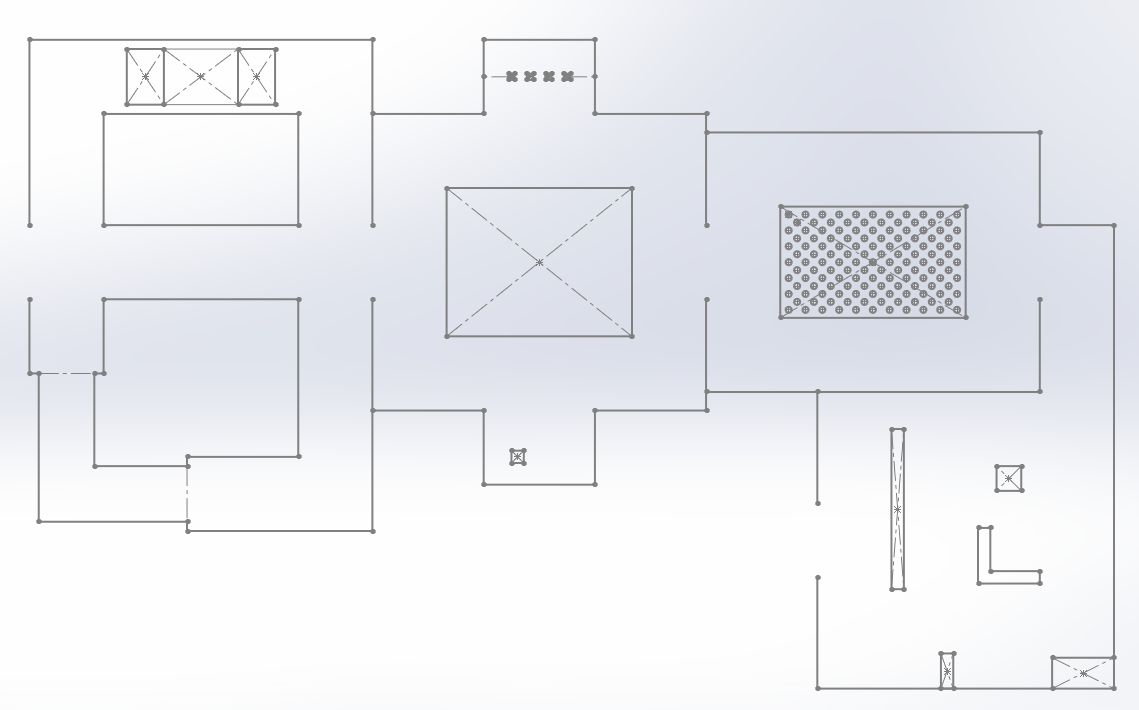
\includegraphics[width=.85\textwidth]{images/track_overview_wlabels.png}
	\caption{Field Overview}
	\label{fig:field} 
\end{figure}

\subsection{Track}
The track is defined as a 24-inch-wide path that is bounded on either side by 3-inch-high walls. The walls used at the competition will be constructed from foam board of the type that is easily obtainable from craft stores: 0.125-inch-thick with a matte, white paper surface. The walls will be stabilized with plastic brackets that will raise them roughly one inch off the floor. The track will be laid out on a terrazzo floor.

\subsection{Bypasses}
The 2020 competition track includes paths that bypass most obstacles. Teams may choose to bypass any or all of the obstacles during a run. See section \ref{bypass} for details.

\subsection{Tunnel}
The tunnel is an L-shaped wooden structure with openings on either end that are 12-inches-high by 18-inches-wide. The interior is dark. This obstacle tests the maneuverability of the robot in a confined space with limited visibility.

\subsection{Bridge}
The bridge is 24-inches-wide with a carpeted surface and no guard walls. The climb is 30-degrees with a 12-inch rise, followed by a 24-inch span and a 30-degree descent. This obstacle tests the robot’s ability to move in a controlled manner on an inclined surface.

\subsection{Object Identification and Handling}
	\subsubsection{Pick-Up Zone}
		There will be four bright red cubes with side lengths of 2 inches in the pick-up zone. Each contains an electromagnetic coil and will be generating a square wave at a unique frequency between 1 Hz and 250 Hz. The robot must detect which object is emitting the field pulsing at 10 Hz. Once detected, the robot is tasked with securing the cube and transferring it to the drop-off zone.
	\subsubsection{Drop-Off Zone}
		There will be one bright yellow bin at the drop-off zone. It will be dimensioned as 4 inches wide by 4 inches deep by 2 inches tall. It will not have a front facing side. The robot is tasked with placing  cube emitting the 10 Hz oscillating signal into the bright yellow bin.

\subsection{Rough Terrain}
The rough terrain section is a 3-feet-wide by 5-feet-long area covered with an array of domes aligned in a diagonal grid pattern. The domes will be 3D-printed plastic with a base diameter of 2 inches and a height of 1/2 inch. There will be walls on the long edges of the section, with bypass paths extending another 24 inches beyond the section walls. This section tests the durability and agility of the robot.

\begin{figure}[H]
	\centering
	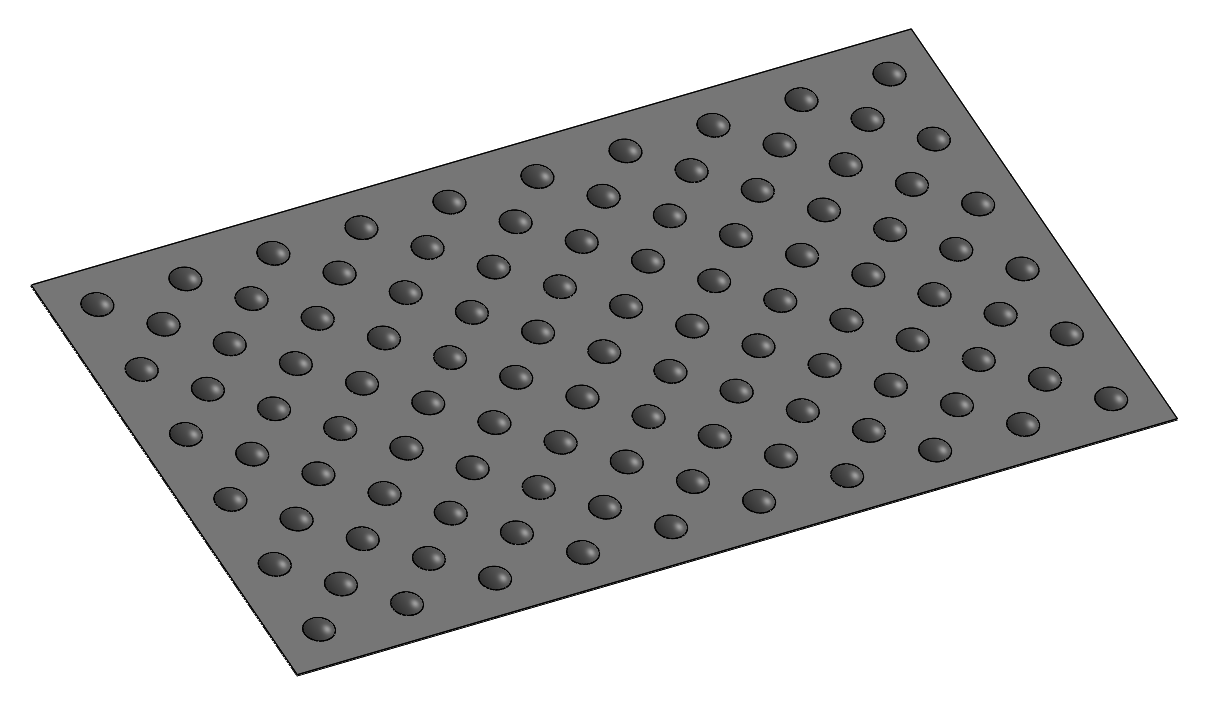
\includegraphics[width=.85\textwidth]{images/rough_terrain.png}
	\caption{Example of Rough Terrain Section}
	\label{fig:rough_terrain} 
\end{figure}

\subsection{Obstacle Avoidance}
The obstacle avoidance section is defined as a rectangular area 6-feet-wide by 8-feet-long. The robot must navigate from the start to the finish without contacting walls or obstacles. Obstacles will consist of standard commercial 2x4 wooden boards varying in length. Note that the actual dimensions of a standard 2x4 are 1.5 inches by 3.5 inches. They will be bright orange. There will be at least one path through this section providing a minimum of 24 inches between obstacles. Three different versions of this section are available; they very in the amount of robot autonomy involved. When registering for the competition, teams will be required to specify which version of the section they wish to attempt. This selection may be changed at or before registration the day of the competition. The three versions of the section are as followed:

\begin{itemize}
    \item Manual - Known Placement
    
        The network will remain enabled and the operator will have full control of the robot as it navigates the section. If this option is chosen, the section will be laid out as defined below.
    \item Autonomous - Known Placement
    
        The network will be disabled and the operator will lose contact with the robot. The robot must be able to navigate the section autonomously. If this option is chosen, the section will be laid out as defined below.
    \item Autonomous - Unknown Placement
    
        The Network will be disabled and the operator will lose contact with the robot. The robot must be able to navigate the section autonomously. If this option is chosen, the layout of obstacles in the section will be unknown to teams until after the deadline to submit robots on the day of the competition. 
        
\end{itemize}

\begin{figure}[H]
	\centering
	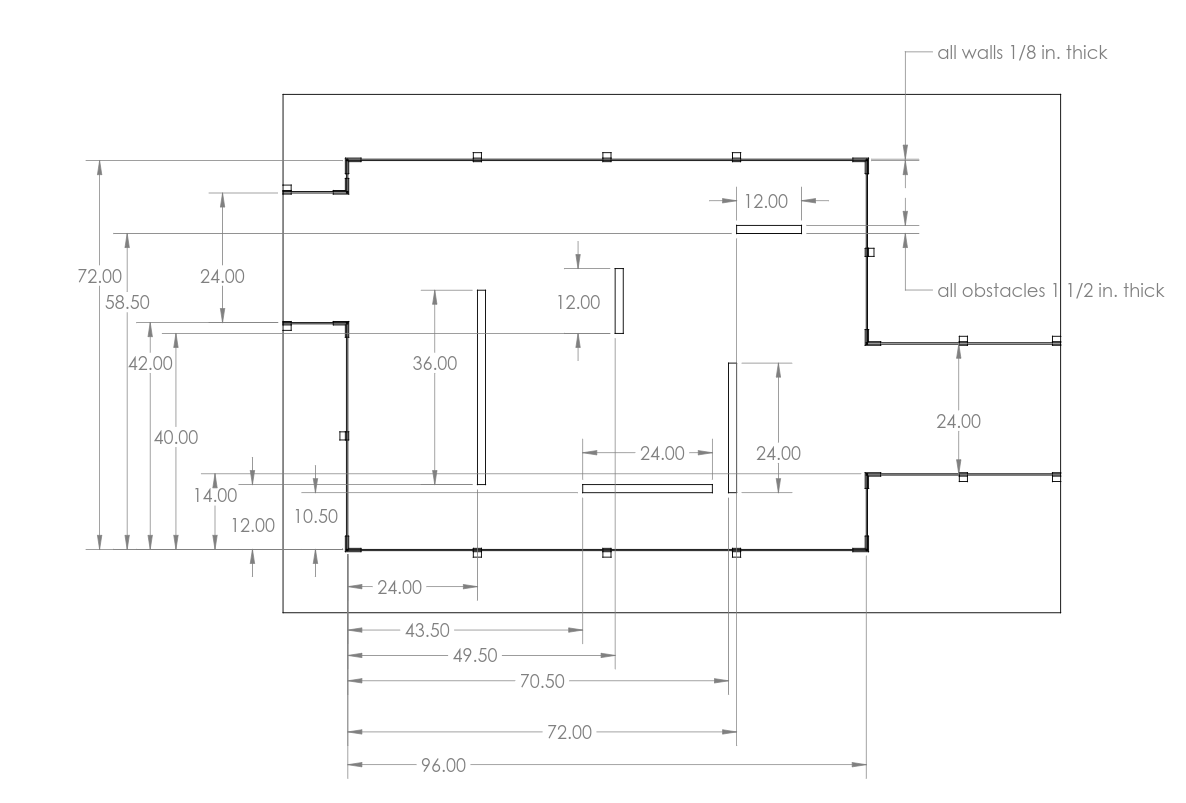
\includegraphics[width=.95\textwidth]{images/avoidance_overview.png}
	\caption{Known Obstacle Layout}
	\label{fig:avoidance_overview} 
\end{figure}